\chapter{General Workflows}\label{sec:general-workflows}


\section{Workflow Recovery}\label{sec:recovery-workflow}

The asynchronous messaging utilizes the guaranteed delivery capability of the message queue platform
to ensure workflows execute to the end even if worker agents are abnormally interrupted.  In most cases,
an abnormal end to an executing process is resumed by the next available worker agent.  
When using an \intlink{sec:external-mq}{external message queue}, this allows for the \cxoneflow endpoint services and
any workflow agents to be recycled without losing workflow state.

Figure \ref{fig:recovery-flowchart} shows the algorithm that is used
in all workflows handle error recovery.  


\begin{figure}[ht]
    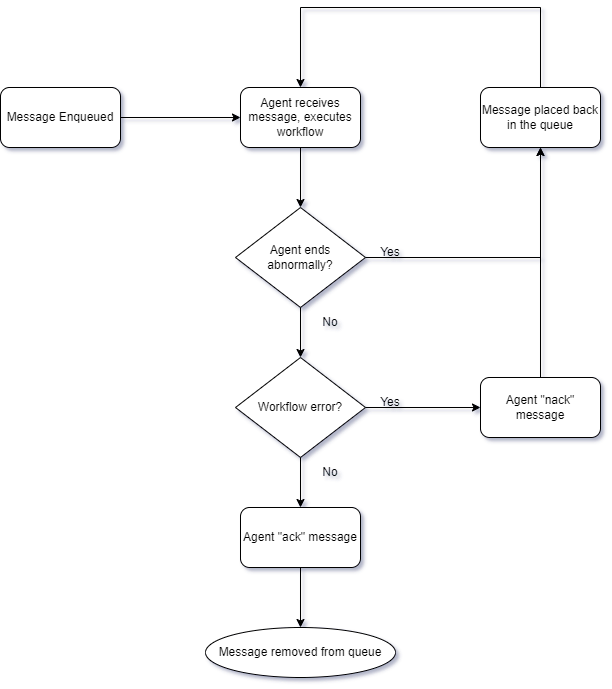
\includegraphics[width=\textwidth]{graphics/cxoneflow-diagrams-Recovery Algorithm.png}
    \caption{Workflow Recovery Algorithm}
    \label{fig:recovery-flowchart}
\end{figure}

